\section{G6: Camera localization}
The goal of this chapter is to localize a calibrated camera relative to a parallelepiped using a single image and known correspondences between \verb|3D| world points and their \verb|2D| projections. The final objective is to determine the camera's extrinsic parameters: the rotation matrix and translation vector, which define the camera's pose in the world coordinate system.

From the previously requests, we know:
\begin{itemize}
    \item the length of the parallelepiped: $l = 1 \, meter$
    \item the depth of the parallelepiped: $m \approx \frac{1}{3} \, meter$
    \item the height of the parallelepiped: $h \approx \frac{1}{2} \, meter$
    \item the camera calibration matrix $K$
\end{itemize}

\paragraph{Reference System}

I decide to consider the following reference system:
\begin{itemize}
    \item X-axis runs along the edge of the length
    \item Y-axis runs along the edge of the depth
    \item Z-axis runs vertically along the edge of the height
\end{itemize}

Defining the \verb|3D| real world points and the respective one in the image, I aim to find the $3 \times 4$ projection matrix which execute the correct mapping.

This is achieved using the Direct Linear Transformation method. It emphasizes constructing the design matrix $A$, solving for $P$ using Singular Value Decomposition (SVD), and interpreting $P$ as the key to extracting the camera's extrinsic parameters.

The \textbf{camera rotation matrix} found is:
\[
    R
    =
    \begin{bmatrix}
        -0.9451 & 0.4853 & -0.0503 \\
        -0.1257 & -0.3673 & -0.9177 \\
        -0.4135 & -0.7935 & 0.3940
    \end{bmatrix}
\]

The \textbf{camera translation vector} is:
\begin{equation}
    t =
    \begin{bmatrix}
        -0.1501 \\
        -0.2444 \\
        -0.7489
    \end{bmatrix}
\end{equation}
   
To enhance the understanding of the obtained result, we visualize the camera within a \verb|3D| model:
\begin{figure}[H]
     \centering
     \begin{subfigure}[b]{0.49\textwidth}
         \centering
         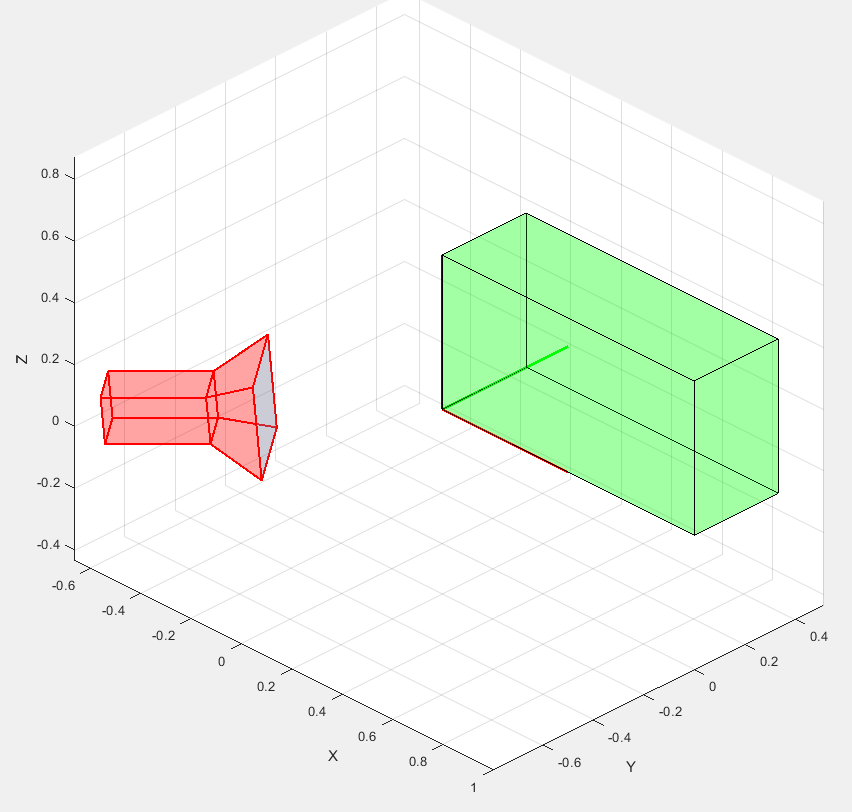
\includegraphics[width=\textwidth]{img/G6/loc1.jpg}
         \caption{Camera localization}
     \end{subfigure}
     \hfill
     \begin{subfigure}[b]{0.49\textwidth}
         \centering
         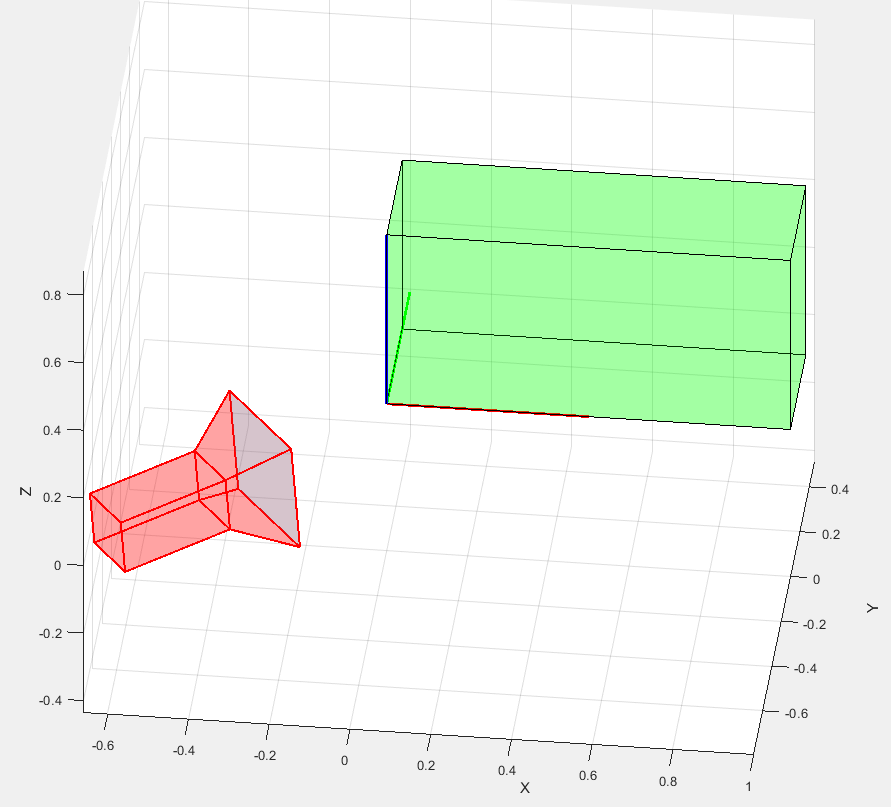
\includegraphics[width=\textwidth]{img/G6/loc2.jpg}
         \caption{Camera localization from a different view}
     \end{subfigure}
\end{figure}